\documentclass[compress,red]{beamer}
\usepackage[utf8]{inputenc}
\usepackage{ucs}
\usepackage{amsmath}
\usepackage{amsfonts}
\usepackage{amssymb}
\usepackage[russian]{babel}
\usepackage{graphicx}
\usepackage{wrapfig}

\usepackage{tikz}
\usepackage{verbatim}

\usepackage{color}
\usepackage{xcolor}
\usepackage{listings}

\usepackage{caption}

\lstset{
language=ruby,
extendedchars=\true,
inputencoding=utf8x,
commentstyle=\itshape,
stringstyle=\bf,
belowcaptionskip=5pt }


\DeclareCaptionFont{white}{\color{white}}
\DeclareCaptionFormat{listing}{\colorbox{gray}{\parbox{\textwidth}{#1#2#3}}}
\captionsetup[lstlisting]{format=listing,labelfont=white,textfont=white}

\usetikzlibrary{calc,trees,positioning,arrows,chains,shapes.geometric,%
    decorations.pathreplacing,decorations.pathmorphing,shapes,%
    matrix,shapes.symbols}

\tikzset{
>=stealth',
  punktchain/.style={
    rectangle, 
    rounded corners, 
    % fill=black!10,
    draw=black, very thick,
    text width=10em, 
    minimum height=3em, 
    text centered, 
    on chain},
  line/.style={draw, thick, <-},
  element/.style={
    tape,
    top color=white,
    bottom color=blue!50!black!60!,
    minimum width=8em,
    draw=blue!40!black!90, very thick,
    text width=10em, 
    minimum height=1.5em, 
    text centered, 
    on chain},
  every join/.style={->, thick,shorten <=1pt},
  decoration={brace},
  tuborg/.style={decorate},
  tubnode/.style={midway, right=2pt},
}

\mode<presentation>

\usetheme{Warsaw}

\definecolor{Red}{rgb}{1,0,0}
\definecolor{Blue}{rgb}{0,0,1}
\definecolor{Green}{rgb}{0,1,0}
\definecolor{magenta}{rgb}{1,0,.6}
\definecolor{lightblue}{rgb}{0,.5,1}
\definecolor{lightpurple}{rgb}{.6,.4,1}
\definecolor{gold}{rgb}{.6,.5,0}
\definecolor{orange}{rgb}{1,0.4,0}
\definecolor{hotpink}{rgb}{1,0,0.5}
\definecolor{newcolor2}{rgb}{.5,.3,.5}
\definecolor{newcolor}{rgb}{0,.3,1}
\definecolor{newcolor3}{rgb}{1,0,.35}
\definecolor{darkgreen1}{rgb}{0, .35, 0}
\definecolor{darkgreen}{rgb}{0, .6, 0}
\definecolor{darkred}{rgb}{.75,0,0}

\xdefinecolor{olive}{cmyk}{0.64,0,0.95,0.4}
\xdefinecolor{purpleish}{cmyk}{0.75,0.75,0,0}

\useoutertheme[subsection=false]{smoothbars}

\title{Кодирование медиа}
\author{Информатика}

%\usecolortheme{dolphin}


\begin{document}
%%титульная страница
\maketitle
%% основные моменты

\section{Кодирование графики}

\subsection{RGB}
\begin{frame}
  \frametitle{RGB}
  \centerline{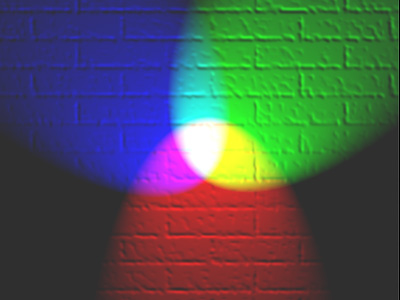
\includegraphics[width=0.8\textwidth]{images/RGB_illumination.jpeg}}
\end{frame}

\subsection{RGB2}
\begin{frame}
  \frametitle{RGB}
  \centerline{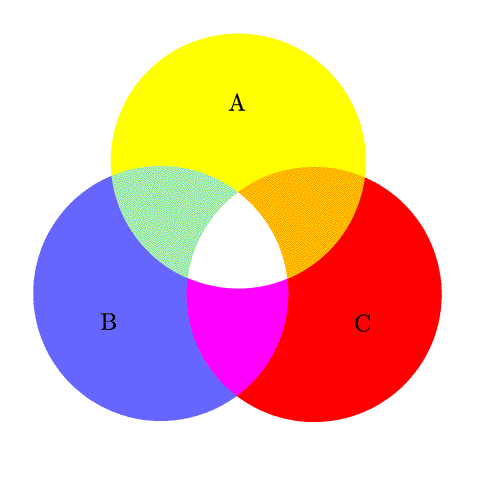
\includegraphics[width=0.7\textwidth]{images/RGB.png}}
\end{frame}

\subsection{RGB3}
\begin{frame}[fragile]
  \frametitle{Описание RGB}
  \begin{itemize}[<+->]
    \item R (red) --- красный,
    \item G (green) --- зелёный,
    \item B (blue) --- синий.
    \item Цвет записывается в виде трёх чисел от 0 до 255: количество красного, количество зелёного, количество синего.
    \item Пример: (255, 0, 0).
  \end{itemize}
\end{frame}

\subsection{RGB4}
\begin{frame}[fragile]
  \frametitle{Примеры цветов}
  \begin{itemize}[<+->]
    \item Красный
    \item (255, 0, 0)
    \item Зелёный
    \item (0, 255, 0)
    \item Синий
    \item (0, 0, 255)
  \end{itemize}
\end{frame}

\subsection{RGB5}
\begin{frame}[fragile]
  \frametitle{Примеры цветов}
  \begin{itemize}[<+->]
    \item Белый
    \item (255, 255, 255) --- сумма всех цветов.
    \item Чёрный
    \item (0, 0, 0) --- отсутствие цвета.
    \item Жёлтый
    \item (255, 255, 0)
    \item Серый
    \item (100, 100, 100)
  \end{itemize}
\end{frame}

\subsection{RGB6}
\begin{frame}[fragile]
  \frametitle{Цвета RGB}
  \centerline{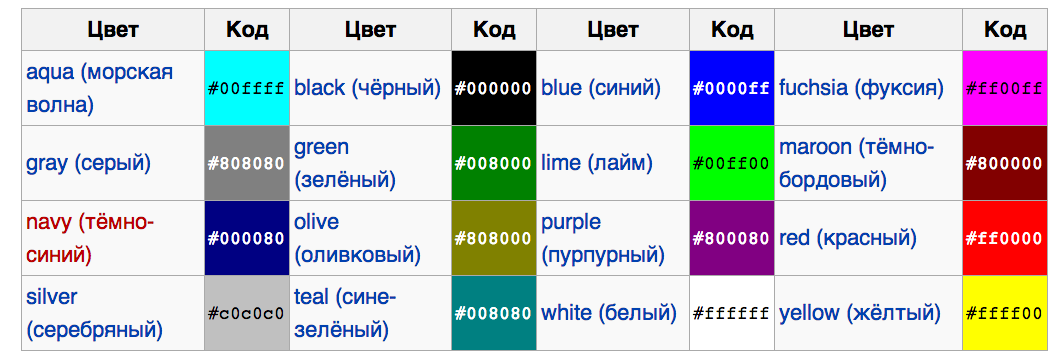
\includegraphics[width=0.7\textwidth]{images/RGB_colors.png}}
\end{frame}

\section{Задачи на графику}
\subsection{Пиксель}
\begin{frame}[fragile]
  \frametitle{Пиксели и их кодирование}
  \begin{itemize}[<+->]
    \item Пиксель --- точка на экране, минимальная единица.
    \item Пиксель представляет собой набор трёх чисел от 0 до 255.
    \item Для кодирования одного числа требуется 8 бит (256 комбинаций).
    \item 3 числа --- $8\cdot 3 = 24$ бита.
    \item Итого, для кодирования 1 пикселя требуется 24 бита.
    \item \textbf{NB:} эти расчёты действуют только для RGB-кодирования. В других случаях 1 пиксель может занимать другое количество бит.
  \end{itemize}
\end{frame}

\subsection{Задача 1}
\begin{frame}[fragile]
  \frametitle{Задача 1}
  \begin{itemize}[<+->]
    \item \textbf{Задача}. Для хранения растрового изображения размером 64 на 64 пикселя отвели 512 байтов памяти. Каково максимально возможное число цветов в палитре изображения?
    \item \textbf{Решение}. Пусть $x$ бит занимает один пиксель данного изображения.
    \item Следовательно, всё изображение займёт $x\cdot 64\cdot 64$~бит $= x\cdot 64\cdot 8$~бит = $ x\cdot 512$~байт.
    \item По условию, всё изображение занимает 512 байт.
    \item Следовательно, $x\cdot 512 = 512$.
    \item $x = 1$ бит.
  \end{itemize}
\end{frame}

\subsection{Задача 2}
\begin{frame}[fragile]
  \frametitle{Задача 2}
  \begin{itemize}[<+->]
    \item \textbf{Задача}. В процессе преобразования растрового графического файла количество цветов уменьшилось с 1024 до 32. Во сколько раз уменьшился информационный объем файла?
    \item \textbf{Решение}. Посчитаем количество бит, которое занимал один пиксель в первом и втором случаях.
    \item В первом случае: для кодирования 1024 комбинаций необходимо 10 бит.
    \item Во втором случае: для кодирования 32 комбинаций надо 5 бит.
    \item Итого, на каждый бит требуется ровно в два раза меньше. Значит, и на все пиксели требуется ровно в два раза меньше.
    \item \textbf{Ответ}: в два раза.
  \end{itemize}
\end{frame}

\subsection{Ещё задачи}
\begin{frame}[fragile]
  \frametitle{Ещё задачи}
  \begin{itemize}[<+->]
    \item Для хранения растрового изображения размером 128 x 128 пикселей отвели 4 килобайта памяти. Каково максимально возможное число цветов в палитре изображения?
    \item Разрешение экрана монитора – 1024 х 768 точек, глубина цвета – 16 бит. Каков необходимый объем видеопамяти для данного графического режима?
    \item В процессе преобразования растрового графического изображения количество цветов уменьшилось с 64 до 8. Во сколько раз уменьшился объем, занимаемый им в памяти?
    \item Сколько памяти нужно для хранения 64-цветного растрового графического изображения размером  32 на 128 точек?
  \end{itemize}
\end{frame}

\section{Кодирование видео и звука}
\subsection{Кодирование видео}
\begin{frame}[fragile]
  \frametitle{Кодирование видео}
  \begin{itemize}[<+->]
    \item Видео --- последовательность картинок. 24(25) кадров/с или другое количество.
    \item Чтобы вычислить информационный объём видео, надо вычислить объём одной картинки, а затем умножить на общее количество изображений.
    \item \textbf{Пример}: оценить информационный объём видео 1024x768 точек, глубина цвета --- 16 бит, 24 кадров/с, которое длится 10 минут.
    \item \textbf{Решение}: $1024\cdot 768$~пикс.~$\cdot 16$~бит~$\cdot 24\cdot 10$~мин.~$\cdot 60$
    \item Полученный ответ будет в битах. Переведём в Мбайты.
    \item $\cfrac{1024\cdot 768\cdot 16\cdot 24\cdot 10}{8\cdot 1024\cdot 1024} = \cfrac{96\cdot 16\cdot 24\cdot 10}{1024} = 360$ Мбайт.
  \end{itemize}
\end{frame}

\subsection{Кодирование звука}
\begin{frame}[fragile]
  \frametitle{Кодирование звука}
  \begin{itemize}[<+->]
    \item \textbf{Задача}. Производится одноканальная (моно) звукозапись с частотой дискретизации 48 кГц и глубиной кодирования 16 бит. Запись длится 2 минуты, ее результаты записываются в файл, сжатие данных не производится. Посчитайте информационный объём в мегабайтах?
    \item Частота дискретизации --- количество возможных комбинаций звука.
    \item Логика решения --- такая же, как и с видео.
    \item \textbf{Решение}. Для хранения 1 секунды видео требуется $48000\cdot 16$ бит.
    \item $48000\cdot 16$~бит$=48000\cdot 2$~байта$=96000$~байт $\approx 0.09$~Мбайт.
    \item Вся запись: $0.09\cdot 2\cdot 60 \approx 11$~Мбайт. 
  \end{itemize}
\end{frame}

\subsection{Задачи на кодирование звука}
\begin{frame}[fragile]
  \frametitle{Задачи на кодирование звука}
  \begin{itemize}[<+->]
    \item Производится одноканальная (моно) звукозапись с частотой дискретизации 22 кГц и глубиной кодирования 16 бит. Запись длится 2 минуты, ее результаты записываются в файл, сжатие данных не производится. Посчитайте информационный объём в мегабайтах?
    \item Производится двухканальная (стерео) звукозапись с частотой дискретизации 48 кГц и глубиной кодирования 24 бита. Запись длится 1 минуту, ее результаты записываются в файл, сжатие данных не производится. Посчитайте информационный объём в мегабайтах?
    \item Производится двухканальная (стерео) звукозапись с частотой дискретизации 11 кГц и глубиной кодирования 16 бит. Запись длится 6 минут, ее результаты записываются в файл, сжатие данных не производится. Посчитайте информационный объём в мегабайтах?
  \end{itemize}
\end{frame}

\end{document}